\documentclass[9pt]{beamer}
\usepackage{beamerthemesplit, pgf, xcolor, graphicx} 
\usetheme{Singapore}
\usecolortheme{seahorse,dolphin}
\usefonttheme{structuresmallcapsserif}

\title{\Huge{
Rare B-Decays to Test The Standard Model and Beyond}}
\author{Becker C., Piscopo M.L., Vlahos C. }

\date{
Supervisors: Krauss F., Maitre D., Pecjak B., Lenz A.\\[11pt]
28.06.2018\\[20pt]
 \begin{columns}
 \begin{column}{0.2 \textwidth}
 
\includegraphics[scale=0.7]{DU_logo.png}
 \end{column}
 \begin{column}{0.3 \textwidth}
 
\includegraphics[scale=0.8]{logo.png}
 \end{column}
 \end{columns}
 }


\begin{document}

\frame{\titlepage}



\frame
{
\frametitle{The Theoretical framework}
The Standard Model (SM) is an elegant and successful theory, though not complete: 
\\[10pt]
\begin{itemize}
\item{The mathematical description stops to be well defined at very high energy scale (experimentally unaccessible).}\\[10pt]
\item{New Physics is also expected at much lower scales, like the ones that the Large Hadron Collider (LHC) is currently (and in future) probing.}\\[10pt]
\item{Discrepancies between theoretical predictions and experiments give a great opportunity to understand the underlying patterns of SM physics and investigate possible new scenarios.}\\[10pt]
\item{ Anomalies have already been found and many more might hide in the huge amount of data that still need to be analyzed. }
\end{itemize}
}

\frame
{
\frametitle{The Theoretical framework}
\begin{itemize}
\item{The central question is how to describe the interaction between two or more particles!?}\\[10pt]
\item{It turns out that there's no analytical finite solution, even in the simplest case..}\\[10pt]
\item{ but it also turns out that most of the time are satisfied conditions that allow to treat this very complex problem as a sum of smaller and more tractable processes.}\\[10pt]
\item{This leads to a series expansion, in which each of the pieces is supposed to be less and less relevant $\rightarrow$ the series can be truncated at the desired order (at a hopefully little cost).}
\end{itemize}
}

\frame
{
  \frametitle{ The Standard Model of particle physics}

\begin{center}
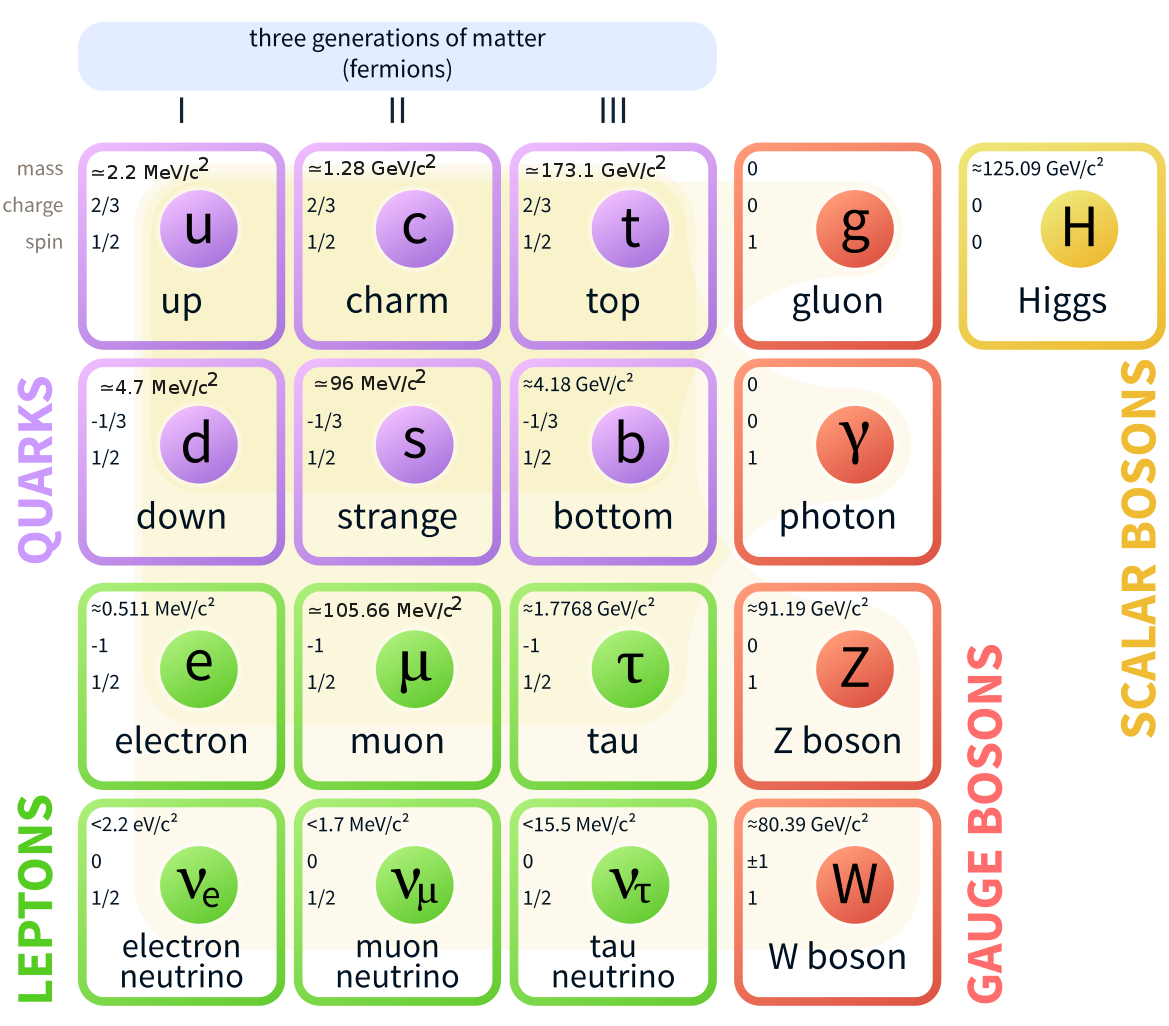
\includegraphics[scale = 0.2]{SM.png}
\end{center}
}



\frame
{
  \frametitle{ The Standard Model of particle physics}

\begin{center}
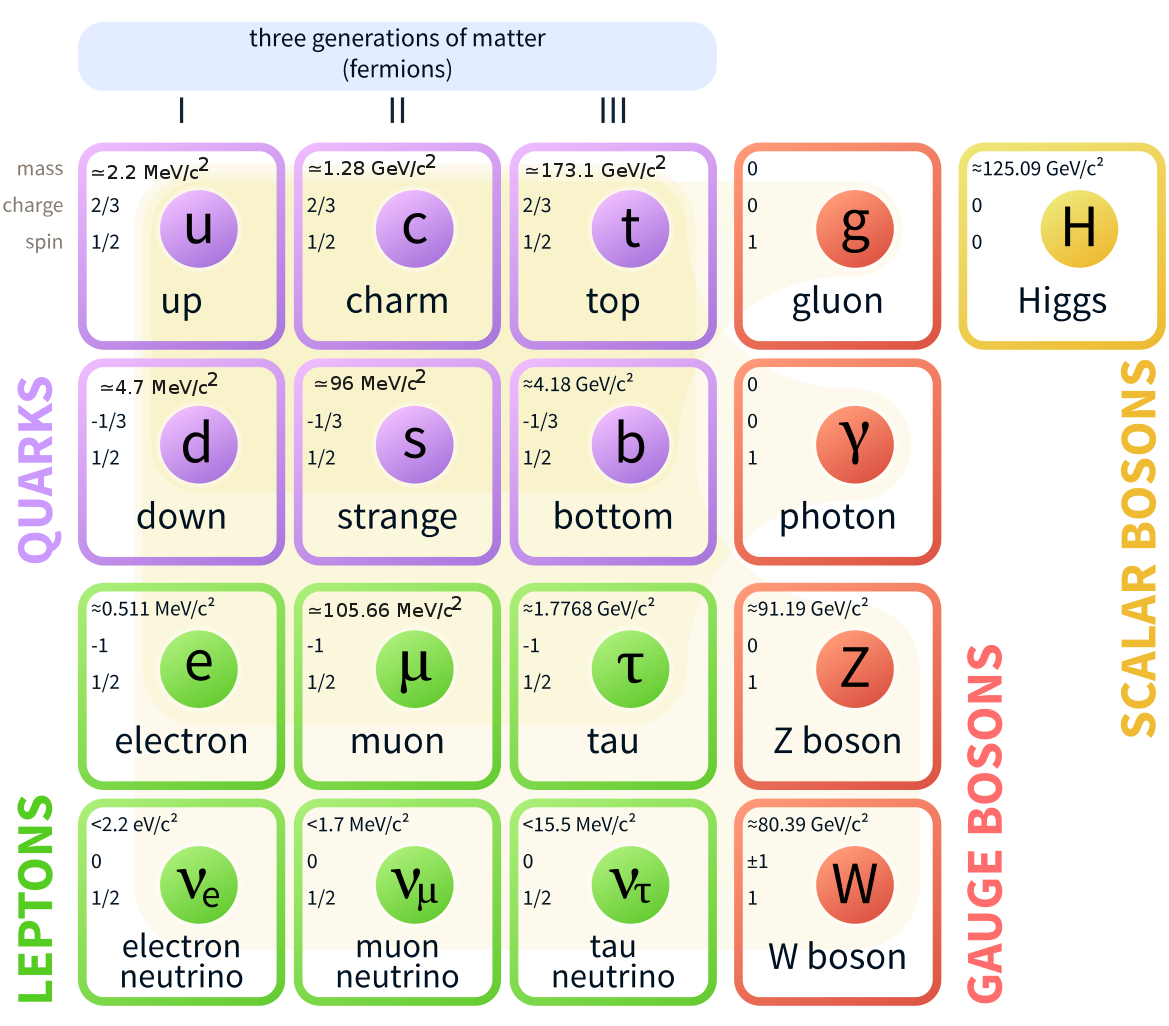
\includegraphics[scale = 0.2]{SM.png}
\end{center}
}

\frame
{
\frametitle{The Theoretical framework}

}




\frame
{
\begin{center}
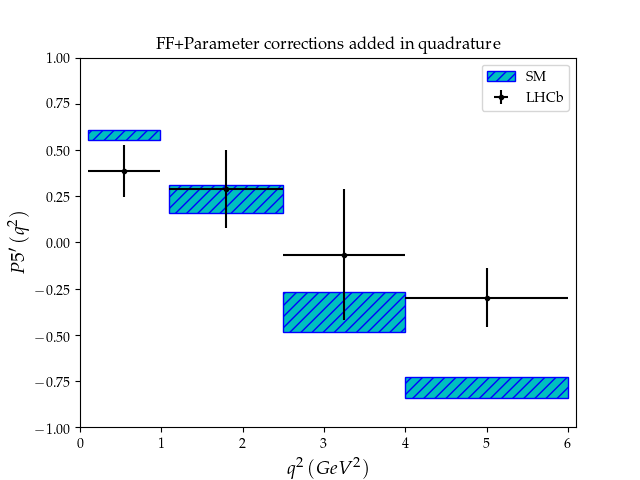
\includegraphics[scale = .7]{FF.png}
\end{center}
}


\end{document}

